
\chapter{Landmarks}
\minitoc 


As stated above, landmarks can be set on surfaces by pressing ``L" + left mouse click. Several actions
can be performed on landmarks.

\section{Select a given landmark.}


\noindent
\begin{minipage}{0.5\textwidth}
When opening the ``select landmark" window, you can
select a given landmark. This option may be useful when
you have digitized many landmarks and/or when some
landmarks become difficult to see.
\end{minipage}    
\begin{minipage}{0.5\textwidth}\centering
  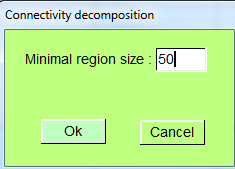
\includegraphics[scale=0.5]{images/Edit_selected_objects/03_Decompose.png}
 \captionof{figure}{Select landmark window}
 \end{minipage} 
\noindent

\section{Select a given range of landmarks.}

Select landmark range window

By opening the ``select landmark range" window, you can
select a given range of landmarks. This option may be useful
when you need to save only a a specific sub-range of all
digitized landmarks.

\section{Push back selected landmarks on closest surface.}
When set via pressing ``L" + left click, landmarks are positioned on one surface’s vertex. Selected
landmarks can be subsequently moved manually to other locations (for instance, if you want to place
a given landmark in the middle of a canal or a foramen, or between two unfused bones). However,
you may sometimes want to push back automatically some selected landmarks to the position of the
closest surface’s vertex available. This can be achieved using this option.


\section{Edit all selected flag landmarks.}
Using this option, you can modify the length and the colour
of several selected flag landmarks at once.

Edit all selected flags window


\section{Change selected landmarks orientation according to surface normals.}
When set via pressing ``L" + left surfaces, landmark orientation is that of the vertex on which it is
placed. Selected landmarks’ orientation can be subsequently moved manually. However, you may
sometimes want to reset one or several landmarks’ orientation automatically to that of the closest
surface’s vertex available. This can be achieved using this option.



\section{Landmarks involved into curves.}

\subsection{Move curve handles (selected yellow
landmarks) semi-automatically}
This option allows saving a lot of time when creating
3D Bezier curves with ISE-MeshTools (see ``working
with curves" section for further details regarding curve
implementation and digitization in ISE-MeshTools).


Mode handles window


Case 1: curve handle is associated to a curve
starting point (A), and a following point (B) exists.
Vector is computed, as well as its length
|AB|.


Curve handle associated to A is moved
from point A along . Displacement
length=movement intensity/|AB|.

Case 2: curve handle is associated to a point B
lying between two points (A and C). Vector is
computed, as well as its length |AC|.

Curve handle associated to B is moved
from point B along . Displacement
length=movement intensity/|AC|.

Case 3: curve handle is associated to a curve
ending point (C), and a preceding point (B) exists.
Vector is computed, as well as its length
|BC|.

Curve handle associated to C is moved
from point C along . Displacement
length=movement intensity/|BC|.


Example of curve handles semi-automatic displacement (movement intensity: 25%).

Requirement : at least a handle landmark (``target" landmark) must be selected.
Depending on whether selected curve handles lie within the curve, at the start of the curve or at the
end of the curve, their displacements differ (see Fig. )



\subsection{Normal landmarks (red): define as curve starting points (green)}
Selected landmark will be given flag ``1"


\subsection{Normal landmarks (red): connect to preceding starting points (violet)}
Selected landmark will be given flag ``3".


\subsection{Normal landmarks (red): define as curve milestones (blue)}
Selected landmark will be given flag ``2".

\subsection{Green, blue, violet landmarks: set back to normal landmarks (red)}
Selected landmark will be given flag ``0".


Further information regarding curve use in ISE-MeshTools is available in the section ``Menu File $\rightarrow$
Curves" section and in the tutorial ``working with curves".